\section{Технологический раздел}

В данном разделе описываются средства реализации программного комплекса. Приводятся листинги программных компонентов, графики процесса обучения разрабатываемой нейронной сети.

\subsection{Средства реализации программного комплекса}

\subsubsection{Выбор языка программирования}

Для написания программного комплекса будет использоваться язык программирования Python \cite{python}.

Данный выбор обусловлен следующими факторами:
\begin{itemize}
	\item широкий набор библиотек для работы с нейронными сетями;
	\item возможность тренировать нейронную сеть на графическом процессоре с использованием технологии CUDA \cite{cuda};
\end{itemize}

\subsubsection{Выбор библиотеки глубокого обучения}

Для создания и обучения модели нейронной сети была выбрана библиотека tensorflow \cite{tensorflow} версии 2.3.0. Выбор данной версии обусловлен тем, что версия 2.3.0 является последней версией с поддержкой CUDA 10, которая предоставляется на высоконагруженном кластере NVIDIA DGX2, на котором будет обучаться нейронная сеть.

Кроме того, tensorflow показал себя производительнее, чем pytorch, что является плюсом, так как тренировка модели с tensorflow займет меньше времени, чем с pytorch \cite{ptvstf}.

\subsubsection{Выбор средства реализации машины опорных векторов}

Для реализации классификатора машины опорных векторов будет использована библиотека Scikit Learn. Она предоставляет реализацию машины опорных векторов и требует от пользователя только данные для обучения \cite{scikitsvm}.

\subsection{Реализация программного комплекса}

\subsubsection{Модель UNet}

Реализация модели построена на классической UNet модели с 23 сверточными слоями. В качестве функции активации на всех слоях, кроме последнего, используется ReLU. На последнем слое используется сигмоидальная функция активации. Она является более точной, чем ReLU, но менее быстрой. Именно поэтому для небольшого увеличения точности она используется именно на последнем слое.

В листинге \ref{lst:unet} (приложение 1) приведена реализация модели, отвечающей за сегментацию изображения.

На выходе модель предоставляет маску для изображения, по которой происходит дальнейшее выделение. Пример такой маски приведен на рисунке \ref{fig:mask}.

\begin{figure}[H]
	\centering
	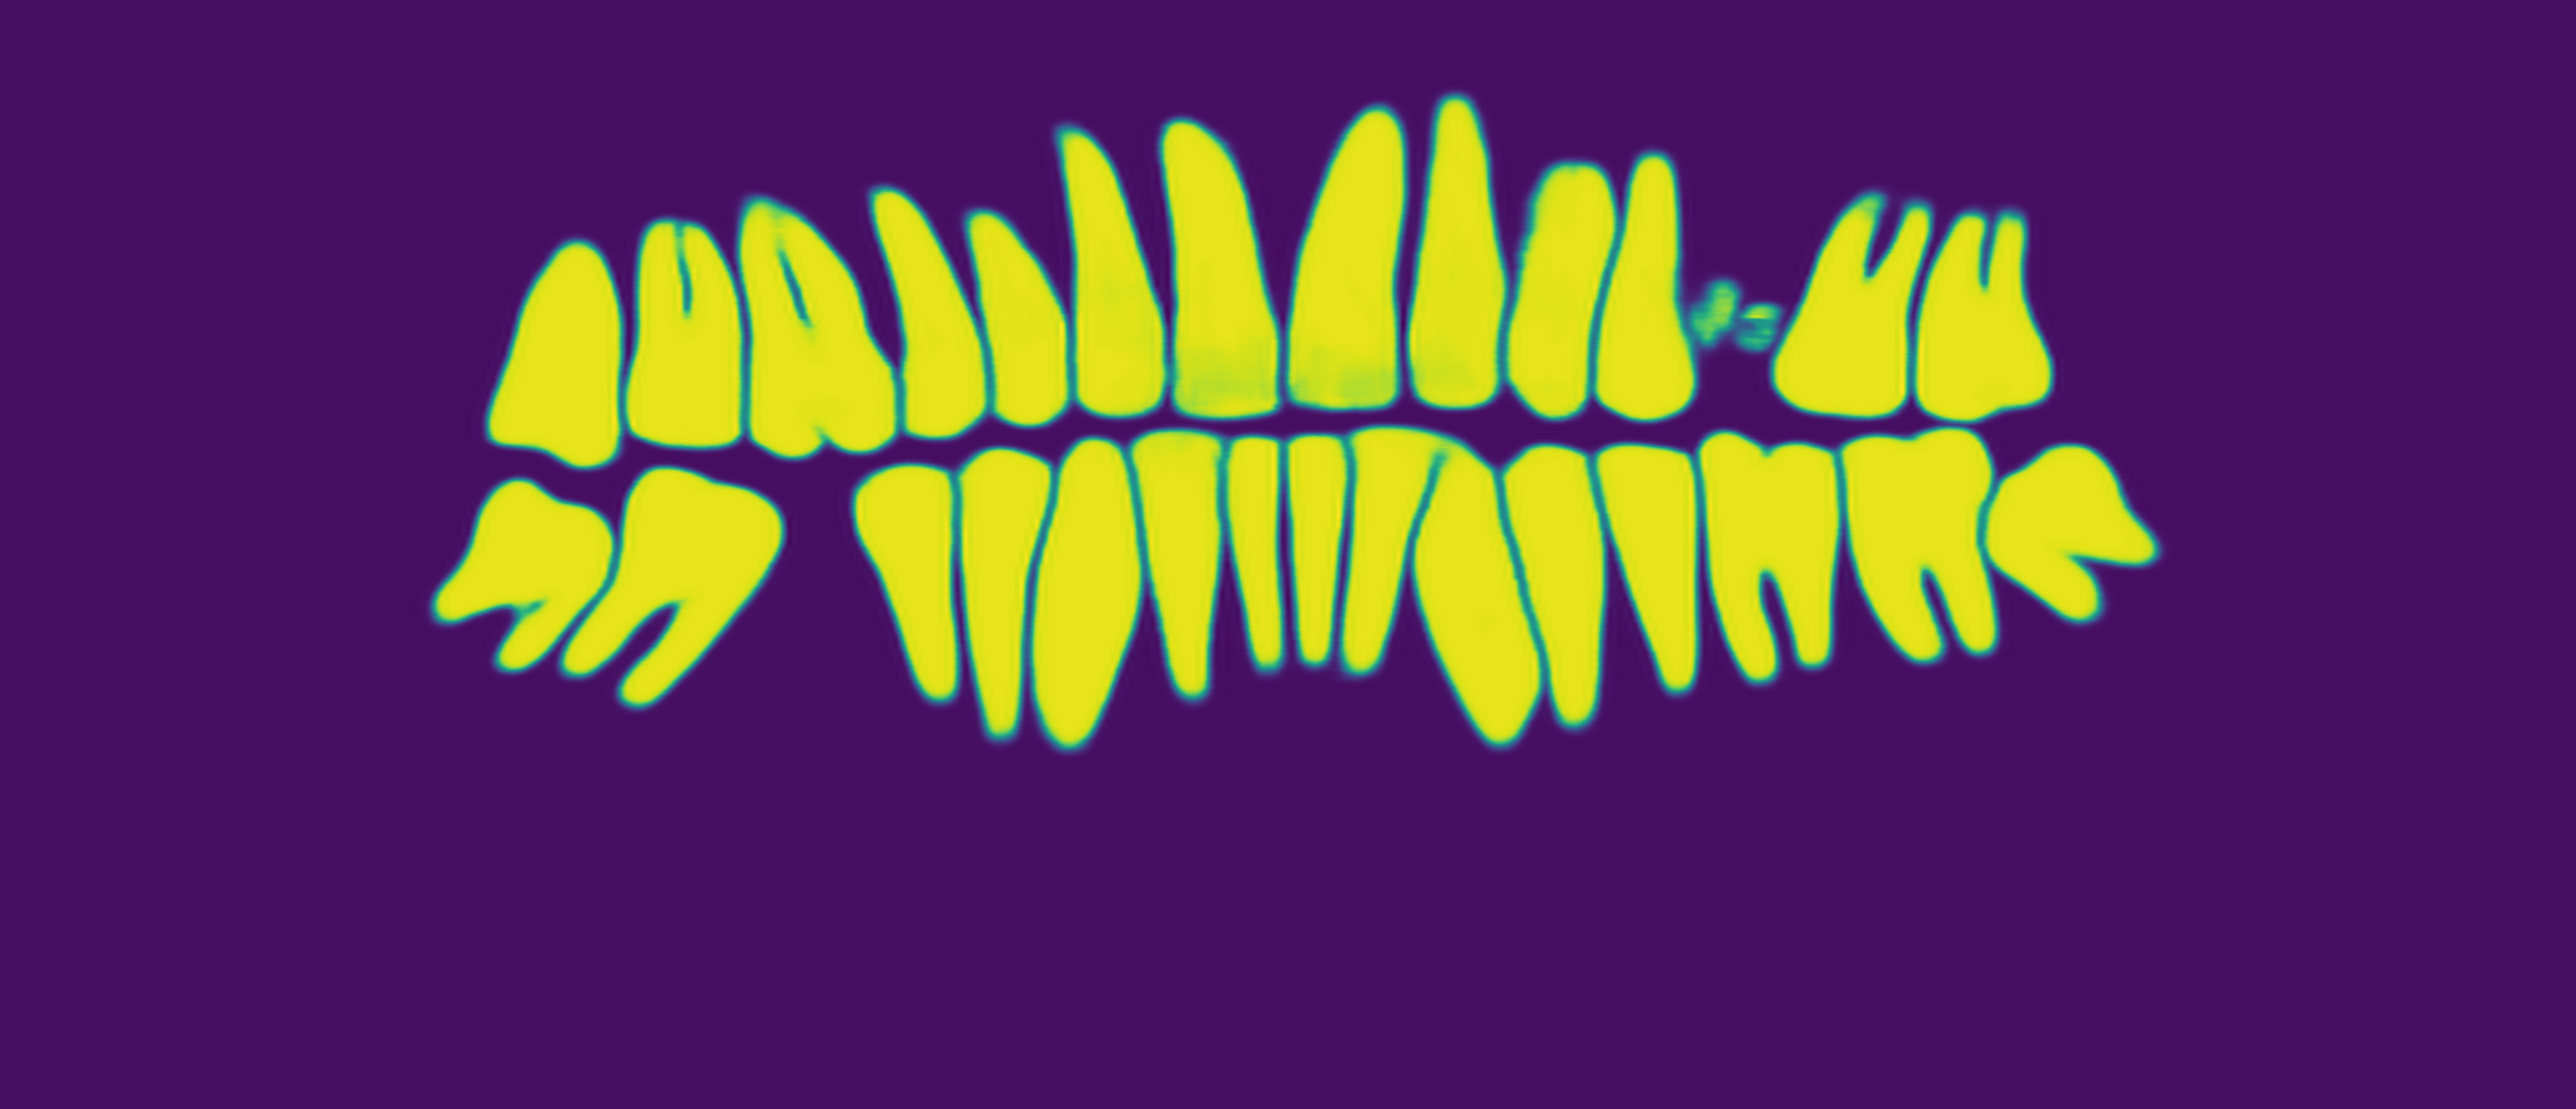
\includegraphics[width=\textwidth]{img/mask.png}
	\caption{Результат работы модели}
	\label{fig:mask}
\end{figure}

\subsubsection{Тренировка модели}

Перед тренировкой модели необходимо произвести конвертацию исходных изображений и их масок к размеру $512 \times 512$ пикселей, как этого требует модель.

Кроме того, в процессе обучения, тренировочные данные подвергаются преобразованиям, таким как обрезка, изменение контраста, поворот, отражения, применение Гауссова шума и прочие. Это нужно для расширения набора тестовых данных и повышения точности модели.

В качестве функции оптимизации для модели будет использована функция Adam (адаптивная оценка момента). Adam --- один из самых эффективных алгоритмов оптимизации в обучении нейронных сетей. Он сочетает в себе идеи среднеквадратичного распространения корня (RMSProp) и оптимизатора импульса. Вместо того чтобы адаптировать скорость обучения параметров на основе среднего первого момента (среднего значения), как в RMSProp, Adam также использует среднее значение вторых моментов градиентов. В частности, алгоритм вычисляет экспоненциальное скользящее среднее градиента и квадратичный градиент.

В листинге \ref{lst:training} (приложение 1)  приведена реализация процесса обучения.

На рисунках \ref{fig:scan} --- \ref{fig:mandible} приведены примеры тренировочных данных для модели: снимок лица, маска зубов и маска нижней челюсти соответственно.

\begin{figure}[H]
	\centering
	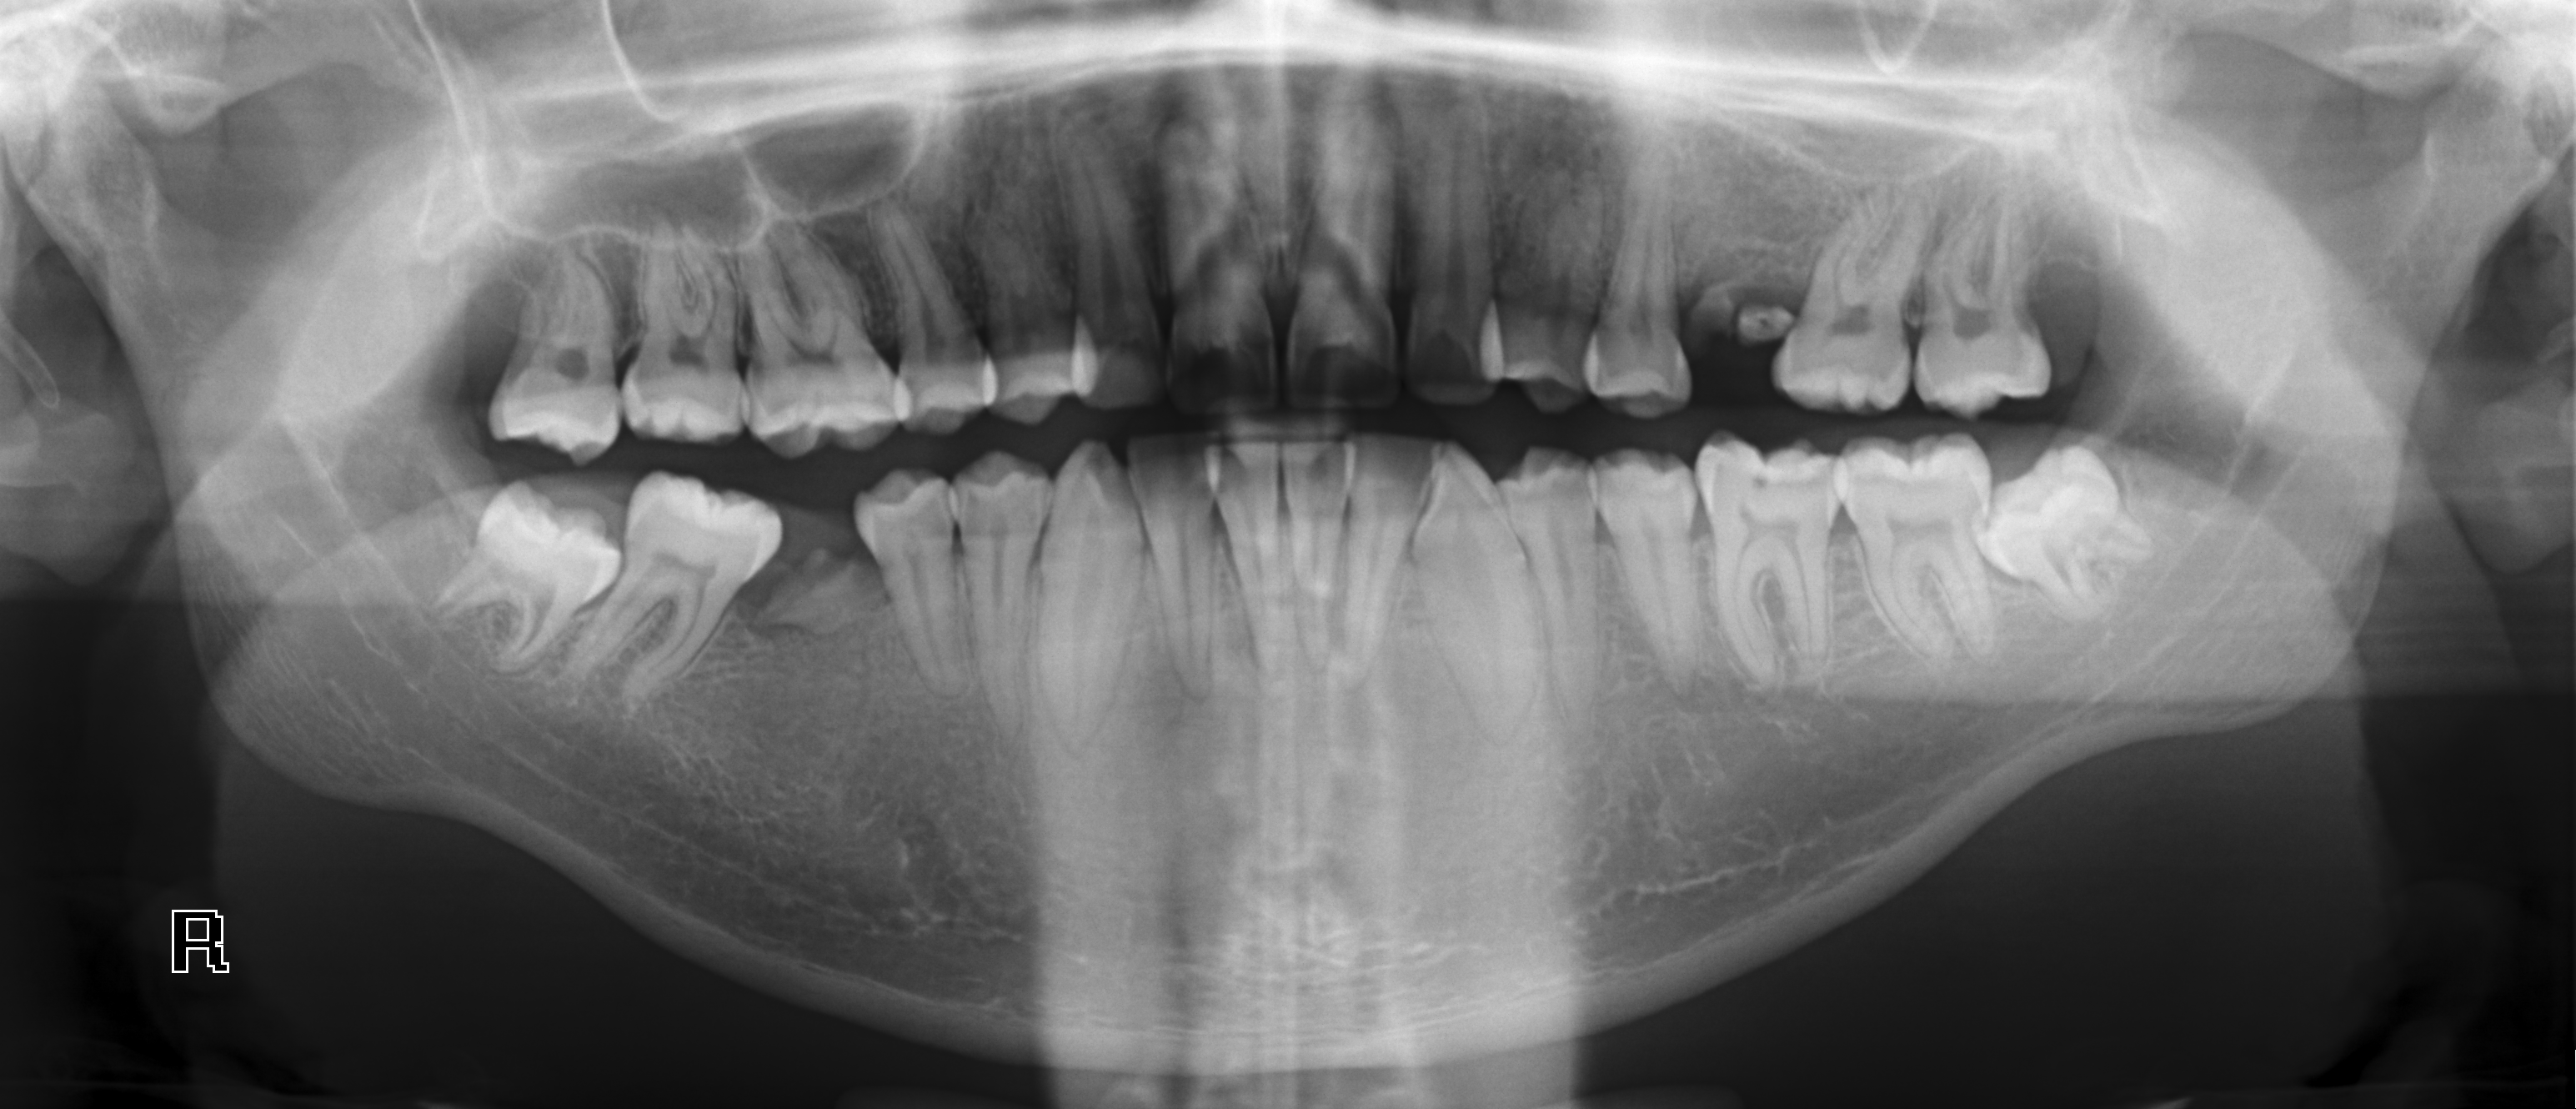
\includegraphics[width=\textwidth]{img/scan.png}
	\caption{Пример тренировочных данных. Томографический снимок}
	\label{fig:scan}
\end{figure}

\begin{figure}[H]
	\centering
	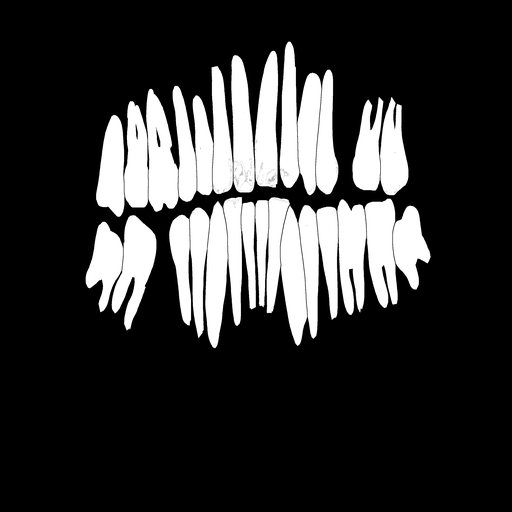
\includegraphics[width=300px]{img/teeth.png}
	\caption{Пример тренировочных данных. Маска зубов}
	\label{fig:teeth}
\end{figure}

\begin{figure}[H]
	\centering
	
\includegraphics[width=300px]{img/mandible.png}
	\caption{Пример тренировочных данных. Маска нижней челюсти}
	\label{fig:mandible}
\end{figure}

Тренировка проходила в течение 200 эпох (итераций) для обеспечения стабильного результата точности и потерь.

\subsubsection{Классификация зубов при помощи машины опорных векторов}

Для реализации машины опорных векторов, используемый датасет был размечен в мануальном режиме. Разметка производилась путем высчета размеров зубов снимков и выделения полученных размеров в четыре группы: моляры, премоляры, улыки и резцы. При формировании векторов особенностей учитывались два фактора: ширина и высота зуба. Вычислить порядковый номер зуба в ряду не представляется возможным в виду представления полученных при сегментации данных.

В листинге \ref{lst:cca} (приложение 2)  приведена реализация и обучение машины опорных векторов.

\subsubsection{Выделение сегментированных участков}

Для выделения сегментированных (и класифицированных) участков используется метод CCA (от англ. Connected Components Analysis --- анализ связанных компонентов). Данный анализ проводится при помощи выделения на изображений объектов переднего плана (сегментированных участков) и последующего анализа полученного участка. Анализ проводится на основе различных факторов, таких как размер, абсолютное и относительное расположение объекта \cite{cca}.

В листинге \ref{lst:cca} (приложение 2)  приведена реализация анализа связанных компонентов с их последующим выделением.

На рисунках \ref{fig:segmented} --- \ref{fig:segmented_svm} представлены изображения с выделенными сегментированными участками.

\begin{figure}[H]
	\centering
	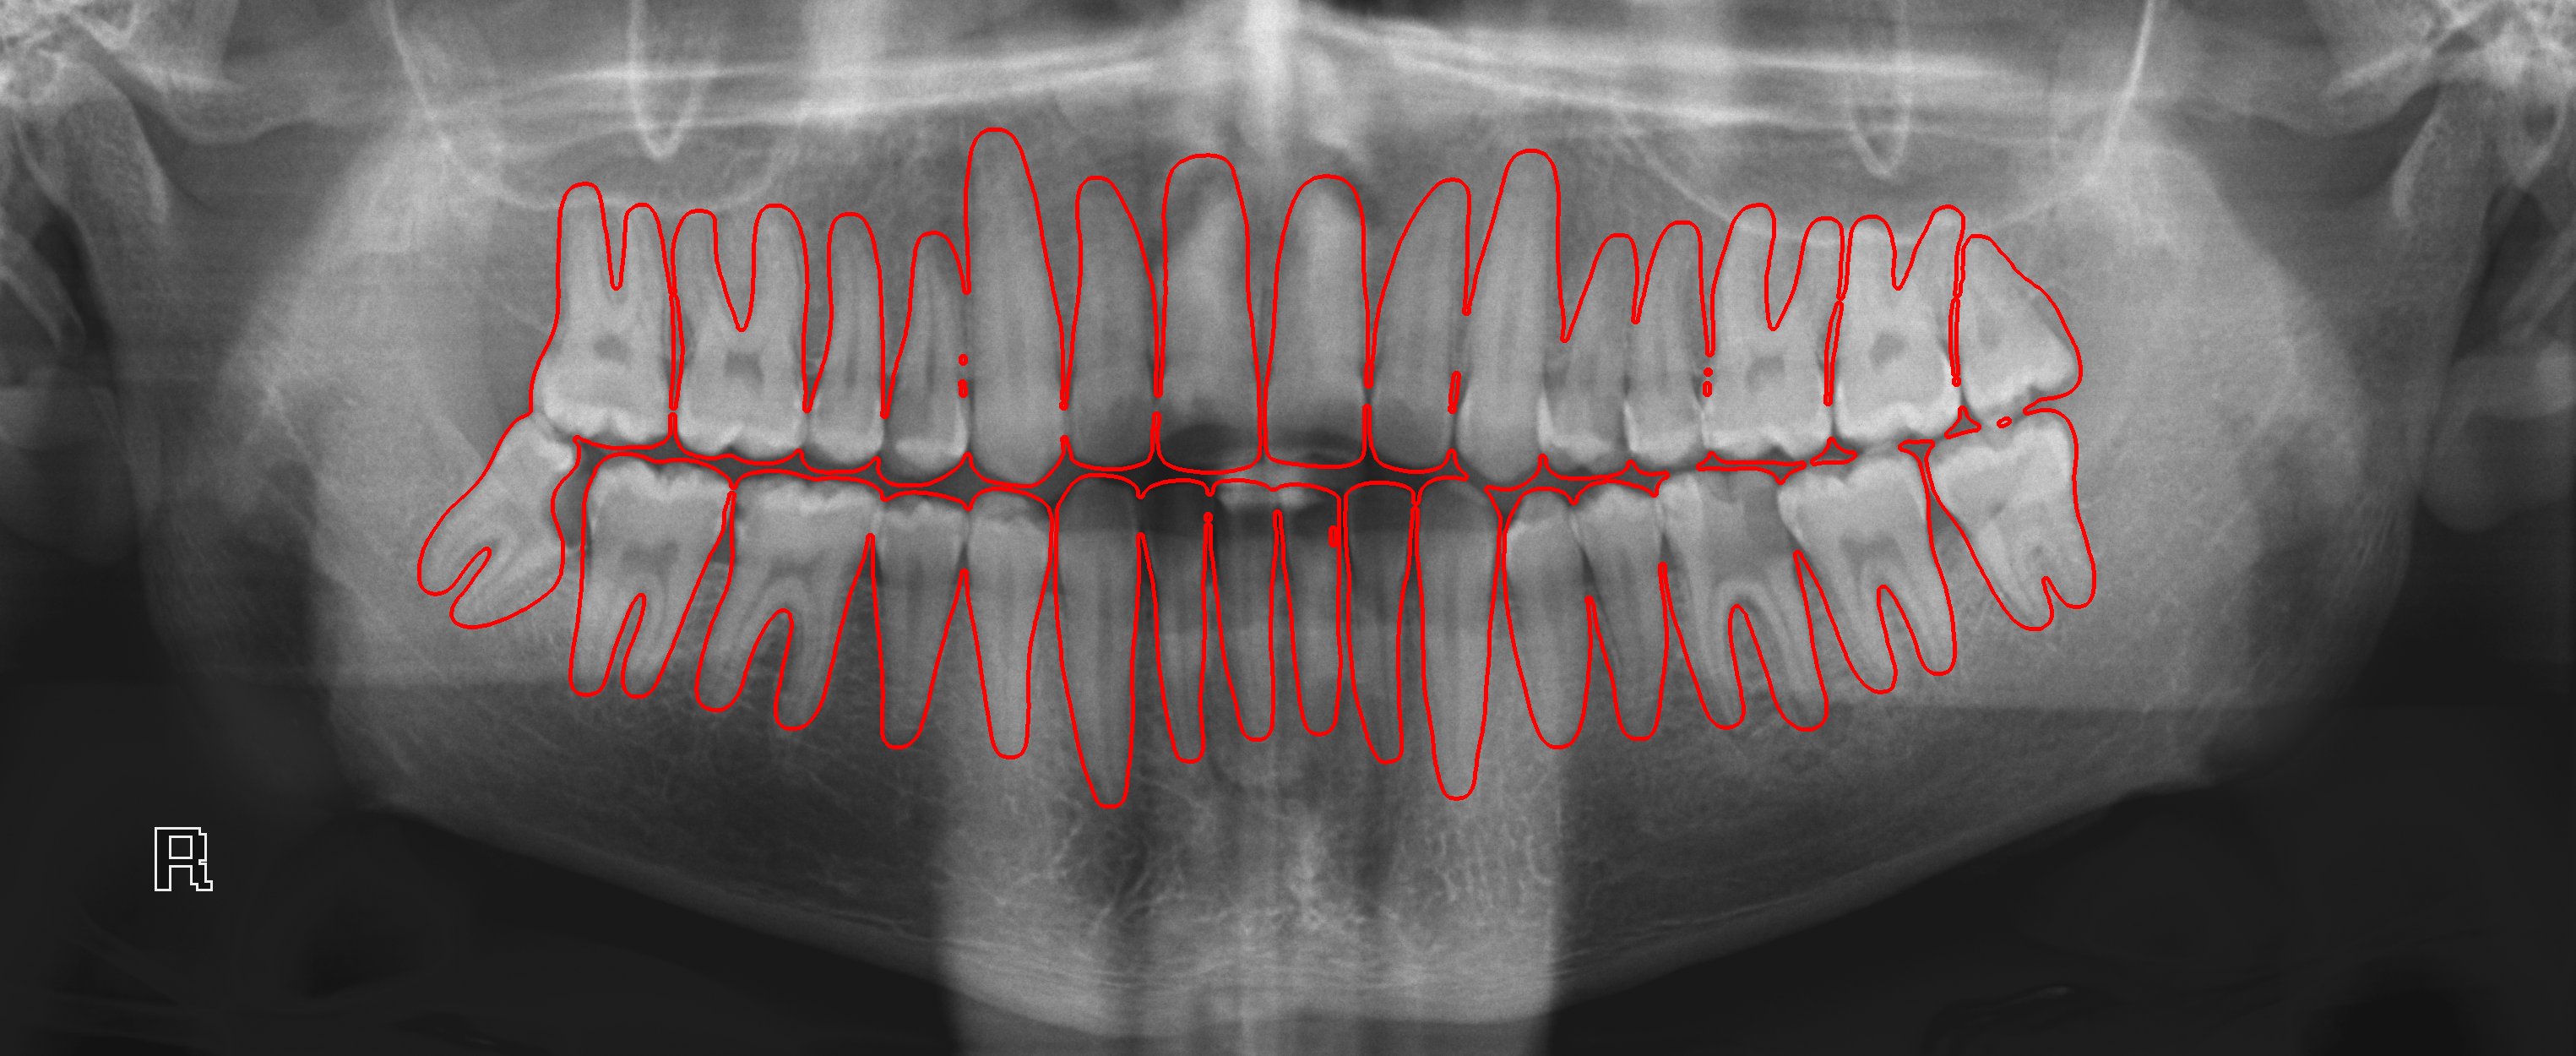
\includegraphics[width=\textwidth]{img/segmented.png}
	\caption{Результат работы семантической сегментации}
	\label{fig:segmented}
\end{figure}

\begin{figure}[H]
	\centering
	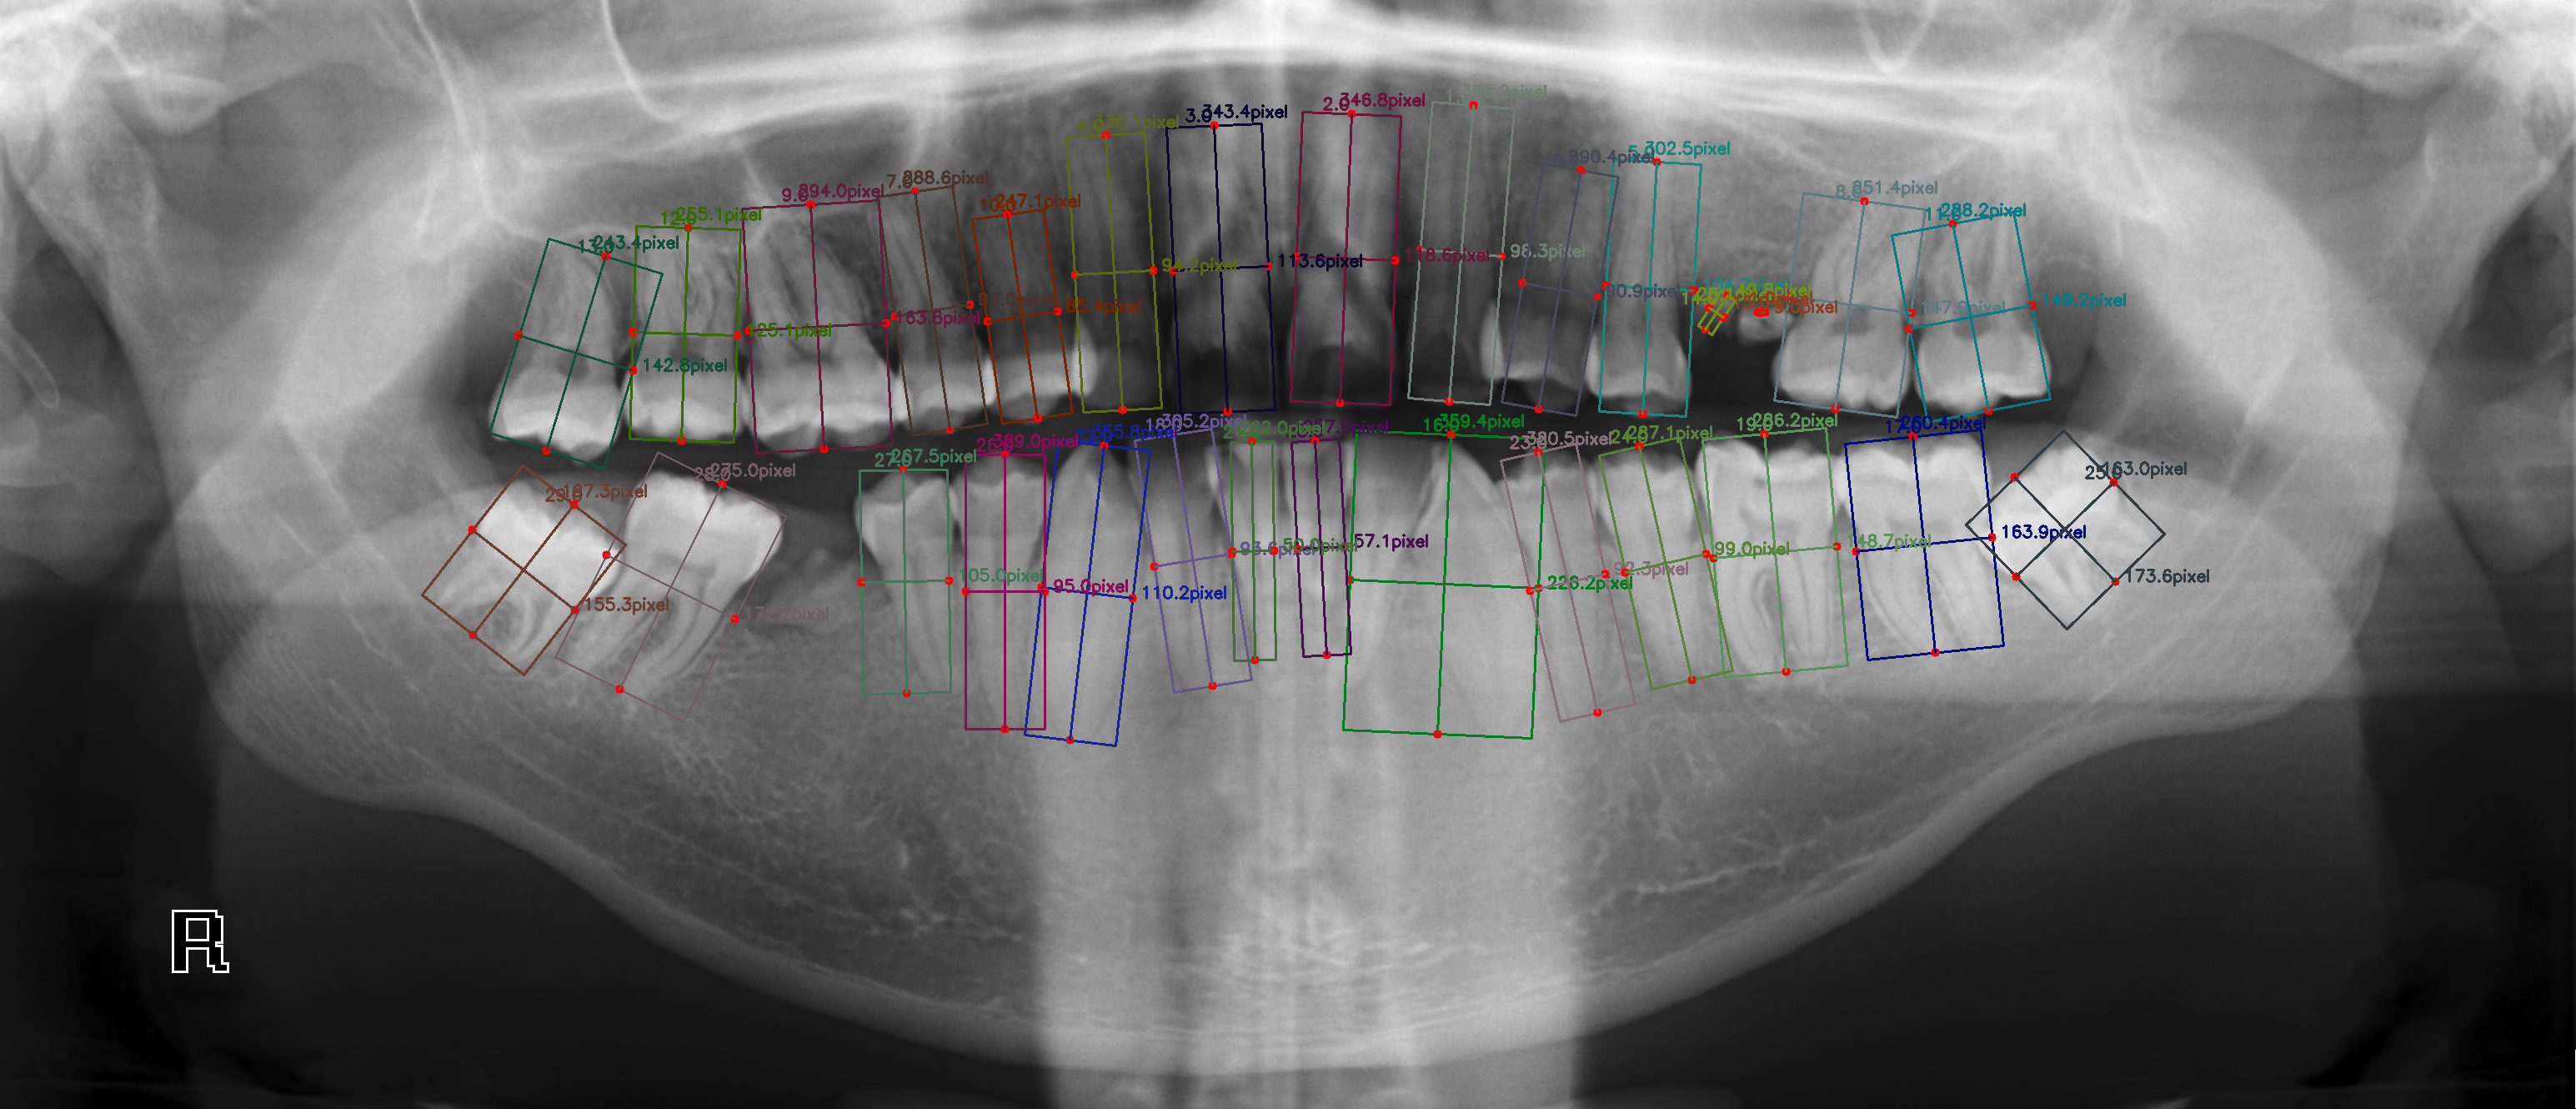
\includegraphics[width=\textwidth]{img/segmented_cca.png}
	\caption{Результат работы сегментации экземпляров}
	\label{fig:segmented_cca}
\end{figure}

\begin{figure}[H]
	\centering
	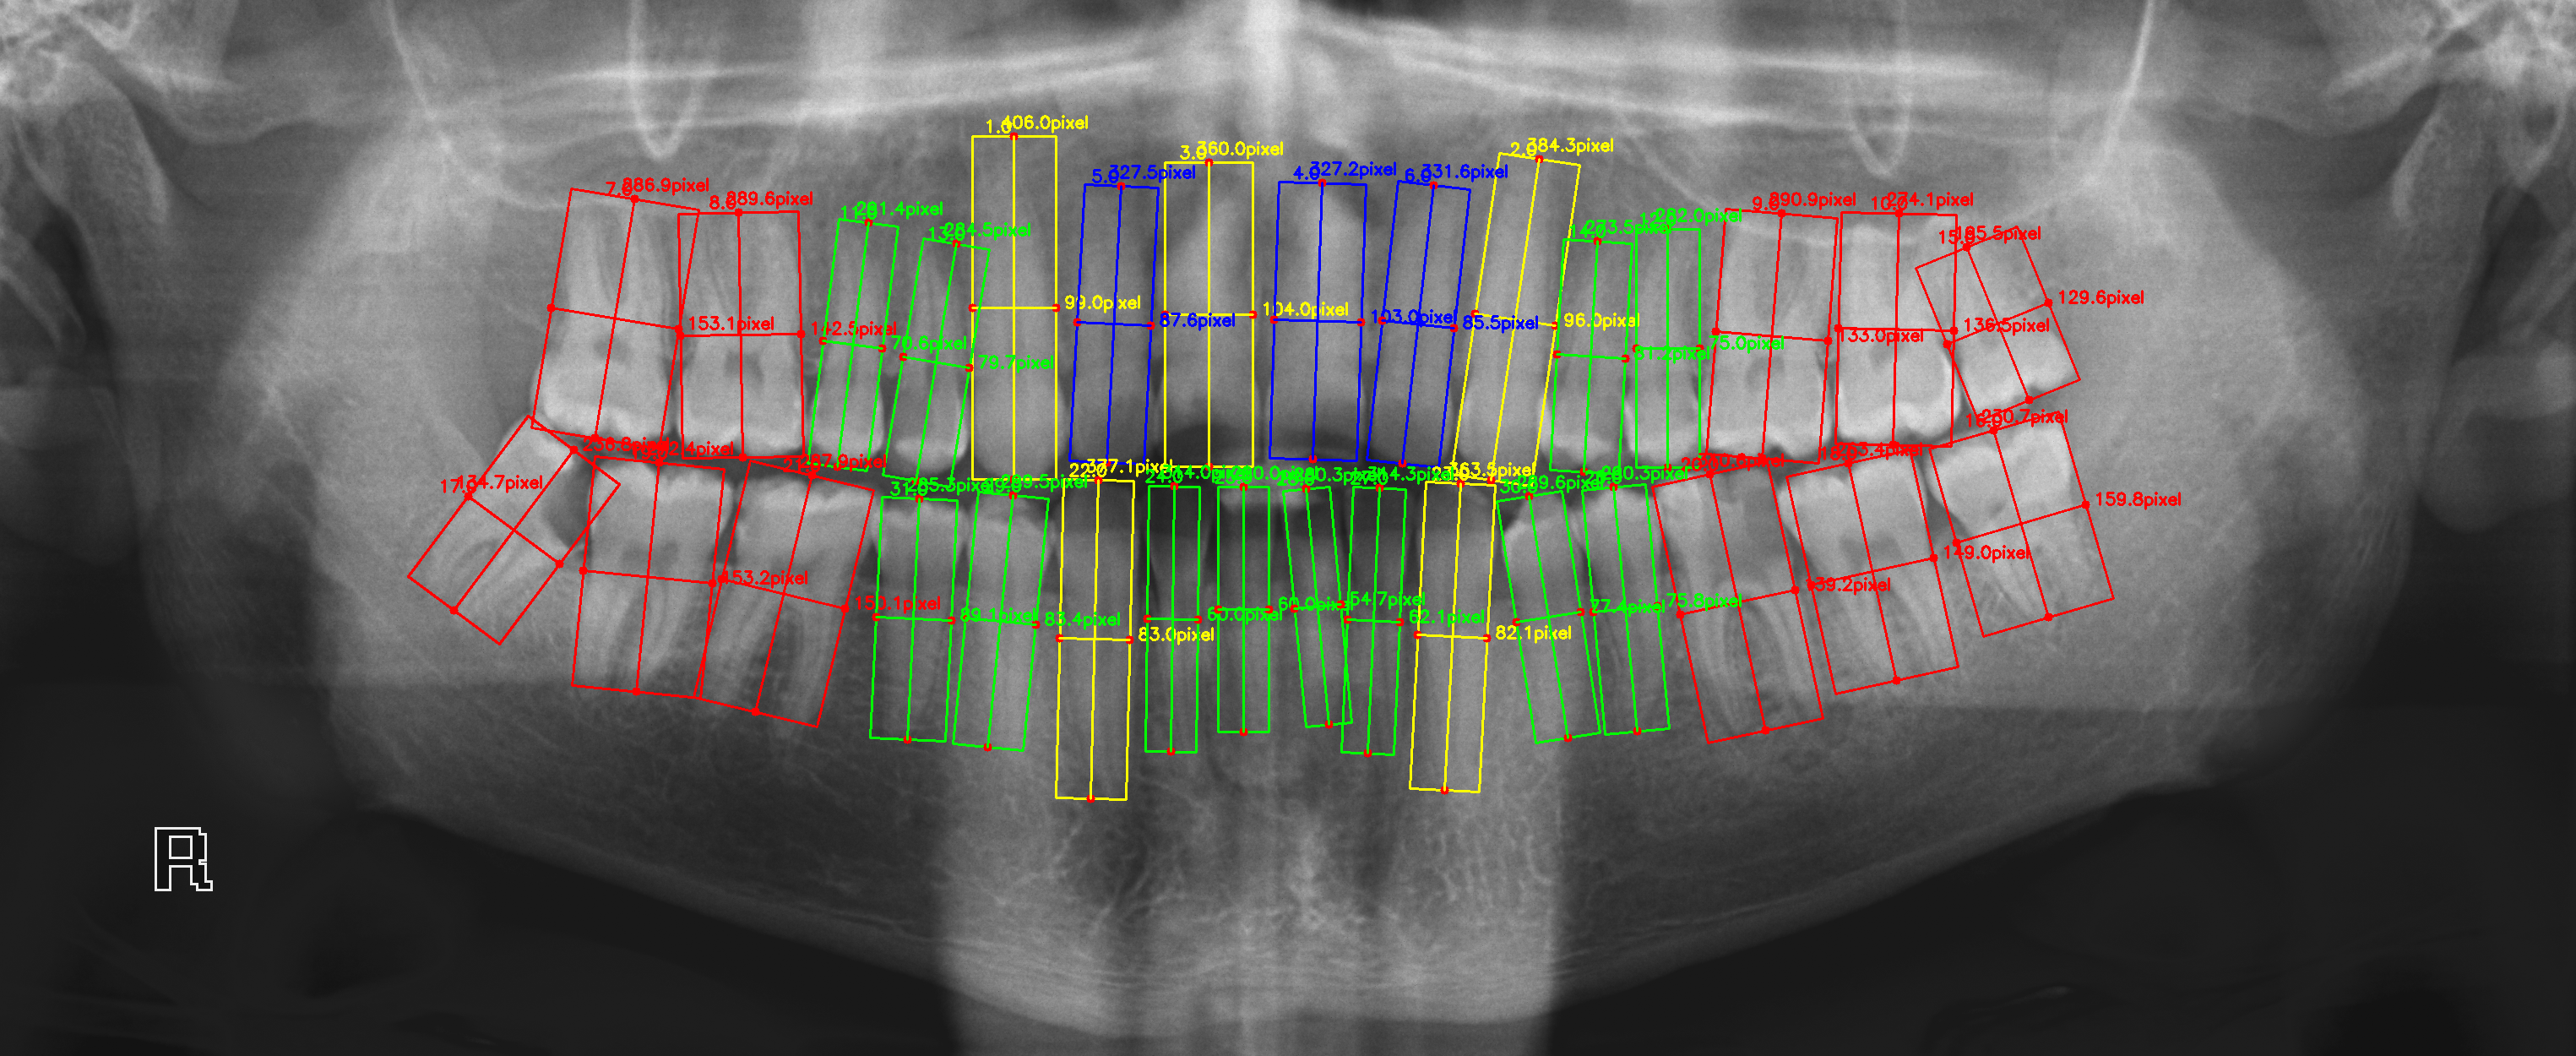
\includegraphics[width=\textwidth]{img/segmented_svm.png}
	\caption{Результат работы сегментации экземпляров (с применением машины опорных векторов)}
	\label{fig:segmented_svm}
\end{figure}

\subsection{Результаты обучения модели}

На рисунках \ref{fig:accuracy} и \ref{fig:loss} представлены результаты обучения модели. Точность модели составила 92 процента, а потери составили 4 процента. Стоит заметить, что уже на десятой итерации точность составила не менее 88 процентов.

\begin{figure}[H]
	\centering
	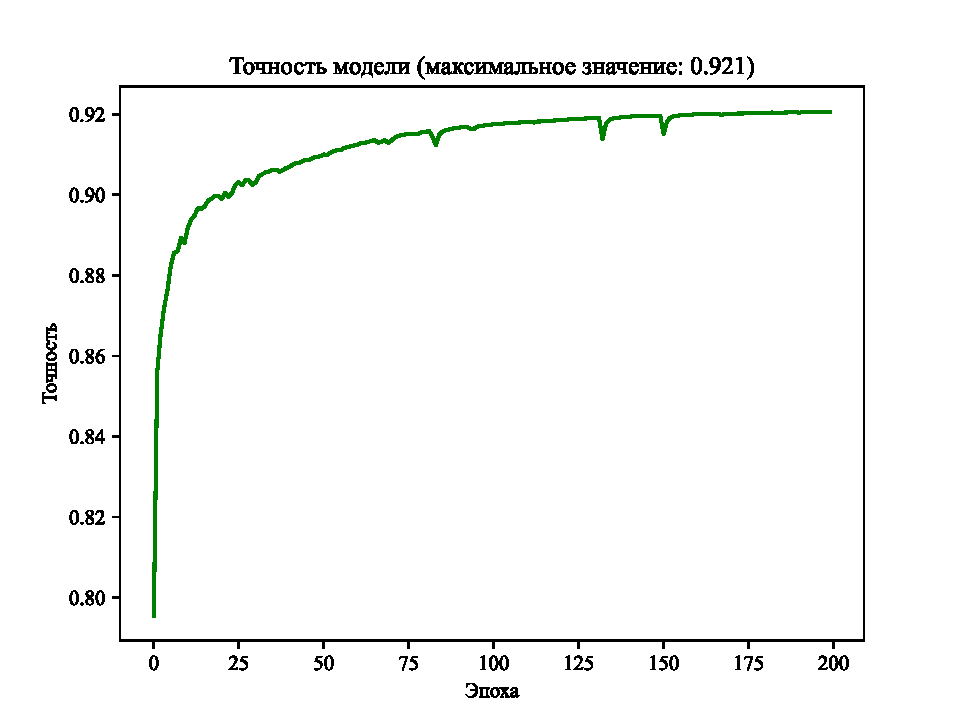
\includegraphics[width=400px]{img/accuracy.pdf}
	\caption{Точность модели}
	\label{fig:accuracy}
\end{figure}

\begin{figure}[H]
	\centering
	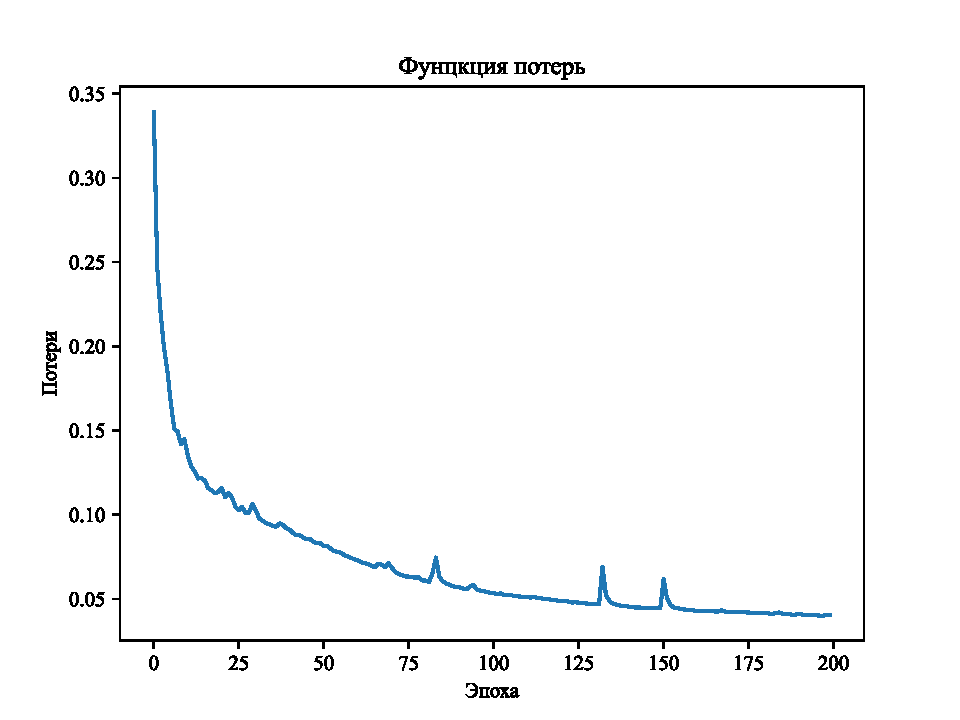
\includegraphics[width=400px]{img/loss.pdf}
	\caption{Потери модели}
	\label{fig:loss}
\end{figure}

\subsection{Примеры использования разработанного программного комплекса}

Оба модуля разработанного программного комплекса представляют собой консольные приложения без графического интерфейса, конфигурируемые при помощи аргументов командной строки.

\subsubsection{Пример использования модуля модели UNet}

В листинге \ref{lst:intmodel} представлены параметры с которыми можно взаимодействовать с модулем обучения модели.

\begin{lstlisting}[
caption={Взаимодействие с модулем модели},
	label={lst:intmodel},
	language=python
]
python main.py -h

usage: main.py [-h] [-m] [-o OUTPUT] [-d DATA]

optional arguments:
-h, --help            show this help message and exit
-m                    Произвести тренировку челюстной сегментации
-o OUTPUT, --output OUTPUT Путь сохранения обученной модели
-d DATA, --data DATA Путь сохранения истории обучения
\end{lstlisting}

В листинге \ref{lst:inttrain} представлены пример запуска модуля для обучения зубной сегментации.

\begin{lstlisting}[
	caption={Запуск обучения},
	label={lst:inttrain},
	language=python
]
python main.py -o trained/teeth.h5 -d trained/teeth.hist

Extracting data/dataset.zip...
Extracted to data
Training teeth segmentation
Extracting masks/teeth.zip...
Extracted to masks/teeth
2022-05-24 01:51:26.391184: I tensorflow/core/platform/cpu_feature_guard.cc:151] This TensorFlow binary is optimized with oneAPI Deep Neural Network Library (oneDNN) to use the following CPU instructions in performance-critical operations:  SSE4.2 AVX AVX2 FMA
To enable them in other operations, rebuild TensorFlow with the appropriate compiler flags.
Epoch 1/200
1/73 [..............................] - ETA: 33:51 - loss: 0.8040 - accuracy: 0.2244
...
\end{lstlisting}

\subsubsection{Пример использования модуля пользовательского приложения}

В листинге \ref{lst:intapp} представлены параметры с которыми можно взаимодействовать с модулем обучения модели.

\begin{lstlisting}[
	caption={Взаимодействие с пользовательским приложением},
	label={lst:intapp},
	language=python
]
python main.py -h

usage: main.py [-h] [-m MODEL] [-i IMAGE] [-o OUTPUT] [-c]

optional arguments:
-h, --help            show this help message and exit
-m MODEL, --model MODEL Путь к файлу с обученной моделью
-i IMAGE, --image IMAGE Пусть к файлу снимка
-o OUTPUT, --output OUTPUT Директория для сохранения результатов
-c                    Произвести сегментацию по экземплярам
\end{lstlisting}

В листинге \ref{lst:intrun} представлены пример запуска приложения с включенной классификацией по типу зубов.

\begin{lstlisting}[
	caption={Запуск приложения},
	label={lst:intrun},
	language=python
]
python main.py -m ../train/trained/teeth.h5 -i ../train/data/Images/19.png -c

2022-05-24 01:57:50.542260: I tensorflow/core/platform/cpu_feature_guard.cc:151] This TensorFlow binary is optimized with oneAPI Deep Neural Network Library (oneDNN) to use the following CPU instructions in performance-critical operations:  SSE4.2 AVX AVX2 FMA
To enable them in other operations, rebuild TensorFlow with the appropriate compiler flags.
Segmented teeth count is 31
\end{lstlisting}

\subsection*{Вывод}

Были описаны средства реализации программного комплекса. Приведены листинги реализации каждого компонента комплекса, примеры работы компонентов, их входные и выходные данные. Описаны технологии и методы, использовавшиеся при реализации. Представлены примеры взаимодействия с модулями.